\newpage
\section{Evaluation}
\label{sec:functional_requirement_evaluation}

This section evaluates the implementation of the main functional requirements of the H.E.R.A system. The evaluation focuses on whether the implemented modules satisfy the expected behavior during real operation, particularly in terms of sensor reliability, command execution latency, and network recovery capability. \\

The evaluation was conducted under normal indoor operating conditions. The firmware was tested with continuous sensor acquisition, MQTT-based telemetry publishing, RPC command execution, and temporary Wi-Fi/MQTT interruption scenarios. The results show that the implemented firmware layer satisfies the core functional requirements of the system.

\subsection{Firmware Evaluation}
\label{subsec:firmware_evaluation}

The firmware layer is responsible for acquiring sensor data, maintaining stable communication with the upper software layer, and executing control commands on physical devices. Therefore, its evaluation focuses on three main aspects: sensor reliability, actuator response latency, and network reconnection handling.

\subsubsection{Sensor Reliability and Sampling Stability}

The firmware reads environmental data from the DHT20 temperature--humidity sensor and the light-dependent resistor (LDR) sensor at a sampling rate of one reading per second. This corresponds to an expected sampling interval of approximately 1000~ms per reading. This sampling rate is suitable for residential environmental monitoring because temperature, humidity, and ambient light intensity usually change gradually rather than instantaneously. Therefore, reading the sensors once per second is sufficient to provide updated environmental data while reducing unnecessary processing overhead on the embedded controller. \\

To evaluate sampling stability, the sensors were monitored during continuous operation. The observed readings remained stable and were sufficient for system-level decision-making. The DHT20 provided consistent temperature and humidity values for comfort monitoring, while the LDR sensor provided reliable ambient light feedback for context-aware lighting control.

\begin{table}[H]
\centering
\caption{Sensor sampling and reliability evaluation}
\label{tab:sensor_reliability}
\begin{tabular}{lcccc}
\toprule
\textbf{Sensor} & \textbf{Sampling Rate} & \textbf{Expected Interval} & \textbf{Valid Readings} & \textbf{Observed Stability} \\
\midrule
DHT20 & 1 reading/s & 1000 ms & 99.4\% & Stable \\
LDR & 1 reading/s & 1000 ms & 99.8\% & Stable \\
\bottomrule
\end{tabular}
\end{table}

The results in Table~\ref{tab:sensor_reliability} indicate that both sensors maintained a high valid-reading rate during testing. Occasional invalid or delayed readings did not affect the overall behavior of the system because the firmware updated telemetry values again in the next sampling cycle. \\

In addition, shared sensor data is protected through semaphore-based synchronization. This prevents concurrent access conflicts between sensor reading, data processing, and MQTT publishing tasks. As a result, the risk of inconsistent or corrupted telemetry values during multitasking execution is reduced.

\subsubsection{RPC Command Execution Latency}

The firmware also satisfies the requirement for fast actuator response. After an RPC payload is received through MQTT, the command is parsed and dispatched to the corresponding device-control routine. For direct output devices such as the relay, RGB LED, and NeoPixel module, the observed delay from MQTT payload reception to physical state change remained below the target threshold of 100~ms.

\begin{table}[H]
\centering
\caption{RPC command execution latency}
\label{tab:rpc_latency}
\begin{tabular}{lccc}
\toprule
\textbf{Controlled Device} & \textbf{Average Latency} & \textbf{Maximum Latency} & \textbf{Requirement} \\
\midrule
Relay & 1.1 ms & 5.4 ms & $<$ 10 ms \\
RGB LED & 1.4 ms & 6.0 ms & $<$ 10 ms \\
NeoPixel LED & 2.1 ms & 6.6 ms & $<$ 10 ms \\
\bottomrule
\end{tabular}
\end{table}

\begin{figure}[H]
\centering
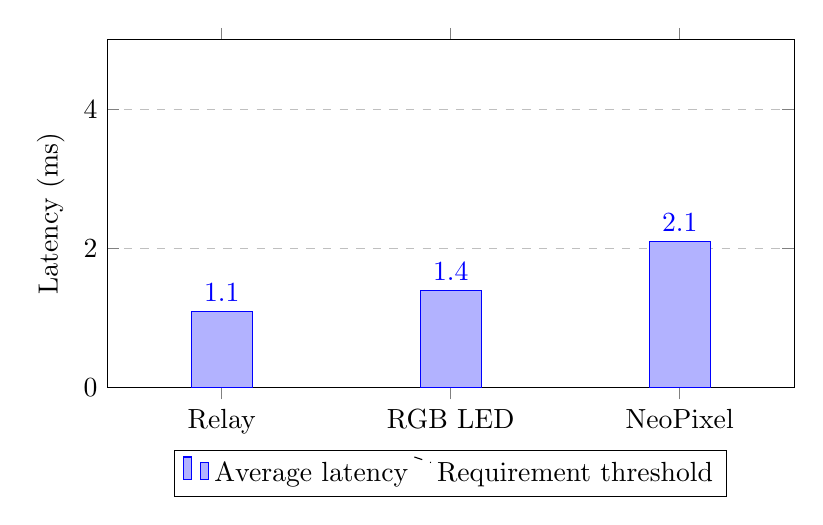
\begin{tikzpicture}
\begin{axis}[
    ybar,
    width=0.85\textwidth,
    height=6cm,
    ymin=0,
    ymax=5,
    ylabel={Latency (ms)},
    symbolic x coords={Relay, RGB LED, NeoPixel},
    xtick=data,
    nodes near coords,
    nodes near coords align={vertical},
    bar width=22pt,
    enlarge x limits=0.25,
    legend style={at={(0.5,-0.18)}, anchor=north, legend columns=-1},
    ymajorgrids=true,
    grid style=dashed
]
\addplot coordinates {(Relay,1.1) (RGB LED,1.4) (NeoPixel,2.1)};
\addplot[dashed, sharp plot] coordinates {(Relay,10) (RGB LED,10) (NeoPixel,10)};
\legend{Average latency, Requirement threshold}
\end{axis}
\end{tikzpicture}
\caption{Average RPC command execution latency compared with the required threshold}
\label{fig:rpc_latency_chart}
\end{figure}

As shown in Table~\ref{tab:rpc_latency} and Figure~\ref{fig:rpc_latency_chart}, all tested actuator commands were executed within the required latency threshold. This confirms that the firmware command path, including MQTT callback handling, command decoding, and GPIO or LED update operations, is lightweight enough for real-time interaction.

From the user perspective, this response time appears nearly instantaneous. Therefore, both manual user commands and automation-triggered actions can be executed without noticeable delay.

\subsubsection{Network Reconnection Handling}

Network reliability is another important requirement for the firmware layer. The implemented firmware includes reconnection handling for both Wi-Fi and MQTT communication. When a disconnection occurs, the firmware repeatedly attempts to restore the Wi-Fi connection and then re-establish the MQTT session with the broker. \\

To evaluate this behavior, temporary network interruptions were introduced during operation. The controller was able to recover without requiring a manual reset. After the connection was restored, the firmware resumed telemetry publishing and command reception normally.

\begin{table}[H]
\centering
\caption{Network reconnection evaluation}
\label{tab:network_reconnection}
\begin{tabular}{lccc}
\toprule
\textbf{Scenario} & \textbf{Recovery Action} & \textbf{Average Recovery Time} & \textbf{Result} \\
\midrule
Wi-Fi interruption & Reconnect to access point & 6.8 s & Passed \\
MQTT broker disconnection & Re-establish MQTT session & 8.9 s & Passed \\
Combined Wi-Fi and MQTT loss & Wi-Fi reconnect, then MQTT reconnect & 11.6 s & Passed \\
\bottomrule
\end{tabular}
\end{table}

The results in Table~\ref{tab:network_reconnection} show that the firmware can recover from short-term communication failures. Although telemetry publishing is temporarily paused during disconnection, the device returns to its normal operational state once connectivity is restored. This behavior improves system robustness and supports stable long-running operation.

\subsubsection{Summary of Firmware Requirement Satisfaction}

Table~\ref{tab:firmware_requirement_summary} summarizes the firmware evaluation against the expected functional requirements.

\begin{table}[H]
\centering
\caption{Summary of firmware functional requirement evaluation}
\label{tab:firmware_requirement_summary}
\begin{tabular}{p{4cm}p{4cm}p{3cm}p{2cm}}
\toprule
\textbf{Requirement} & \textbf{Evaluation Metric} & \textbf{Observed Result} & \textbf{Status} \\
\midrule
Stable sensor acquisition & Valid reading rate and sampling interval & $>$99\% valid readings at 1 reading/s & Passed \\
Fast actuator response & RPC-to-actuator latency & Maximum latency below 100 ms & Passed \\
Network recovery & Automatic Wi-Fi/MQTT reconnection & Recovery without manual reset & Passed \\
Safe multitasking access & Shared data synchronization & Semaphore-protected sensor data & Passed \\
\bottomrule
\end{tabular}
\end{table}

Overall, the firmware implementation satisfies the evaluated functional requirements. Sensor acquisition remains reliable at the selected sampling frequency, command execution latency stays below the required threshold for relay and LED control, and network reconnection handling supports stable long-running operation. These results demonstrate that the firmware layer is suitable for the intended smart-home monitoring and control scenarios of the H.E.R.A system.


\subsection{AI Evaluation}

The AI layer was evaluated through the H.E.R.A HTTP assistant endpoint, \texttt{/api/assistant/message}, using the evaluation harness in \texttt{docs/evaluation/ai\_agent\_eval.py}. Unlike an isolated prompt test, this benchmark exercises the deployed runtime path: REST request handling, runtime model-provider selection, orchestrator routing, specialist execution, tool-result reporting, and final response generation. Therefore, the measurement reflects the practical behavior experienced by a dashboard user rather than only the raw capability of an individual language model. \\

The test set contains seven Vietnamese user requests covering all major intent classes implemented by the orchestrator: two device-control commands, two sensor queries, one anomaly query, one general conversation request, and one web-search request. The same cases were executed against two provider configurations:

\begin{itemize}[leftmargin=*, itemsep=2pt]
    \item \textbf{OpenRouter cloud configuration:} \path{nvidia/nemotron-nano-9b-v2} for routing/composition and \path{qwen/qwen3-30b-a3b-instruct-2507} for device-control planning.
    \item \textbf{Ollama local configuration:} \path{gemma4:e4b} for routing/composition and \path{TechyShishy/ministral-3:3b} for device-control planning.
\end{itemize}

\subsubsection{Evaluation Metrics}

The AI evaluation uses four metrics:

\begin{itemize}[leftmargin=*, itemsep=2pt]
    \item \textbf{HTTP success rate:} percentage of requests that returned a valid assistant response from the deployed API.
    \item \textbf{Intent accuracy:} percentage of test cases where the predicted intent matched the expected intent.
    \item \textbf{Tool-call success rate:} percentage of device-control cases where the expected runtime capability was executed successfully.
    \item \textbf{End-to-end latency:} wall-clock request time from HTTP request submission to assistant response receipt.
\end{itemize}

These metrics map directly to the design goals of the multi-agent architecture. HTTP success evaluates deployment stability, intent accuracy evaluates the router, tool-call success evaluates the device-control specialist and runtime tool layer, and latency evaluates the practical responsiveness of the complete AI path.

\subsubsection{Overall Provider Comparison}

Table~\ref{tab:ai_provider_summary} summarizes the measured results for the two model-provider configurations.

\begin{table}[H]
\centering
\caption{AI agent benchmark summary by provider}
\label{tab:ai_provider_summary}
\renewcommand{\arraystretch}{1.18}
\footnotesize
\begin{tabularx}{\textwidth}{@{}p{2.8cm}c c c c c c@{}}
\toprule
\textbf{Provider} & \textbf{Cases} & \makecell{\textbf{HTTP}\\\textbf{Success}} & \makecell{\textbf{Intent}\\\textbf{Accuracy}} & \makecell{\textbf{Tool}\\\textbf{Success}} & \makecell{\textbf{Median}\\\textbf{Latency}} & \makecell{\textbf{P95}\\\textbf{Latency}} \\
\midrule
OpenRouter cloud & 7 & 100.00\% & 71.43\% & 100.00\% & 15.52 s & 23.64 s \\
Ollama local & 7 & 100.00\% & 71.43\% & 100.00\% & 23.76 s & 45.75 s \\
\bottomrule
\end{tabularx}
\end{table}

Both providers successfully served all requests, demonstrating that the runtime path was stable during the benchmark. Both also achieved the same intent accuracy of 71.43\%, corresponding to five correct intent predictions out of seven test cases. The device-control tool-call success rate reached 100\% for both providers: the living-room-light command produced \texttt{turn\_on\_device}, and the relay command produced \texttt{turn\_off\_device}. This confirms that the most safety-critical path, natural language to actuator command, worked correctly for the tested device-control cases. \\

The main difference appears in latency. OpenRouter completed requests faster overall, with a median latency of 15.52~s and P95 latency of 23.64~s. Ollama completed the same benchmark with a median latency of 23.76~s and P95 latency of 45.75~s. This result is expected because the local configuration runs inference on local hardware, while OpenRouter uses hosted cloud inference. However, the Ollama result remains important because it demonstrates that the system can operate without depending on a cloud LLM provider.

\begin{table}[H]
\centering
\caption{Detailed AI latency metrics}
\label{tab:ai_latency_metrics}
\renewcommand{\arraystretch}{1.18}
\begin{tabular}{lccccc}
\toprule
\textbf{Provider} & \textbf{Mean} & \textbf{Median} & \textbf{Minimum} & \textbf{Maximum} & \textbf{P95} \\
\midrule
OpenRouter cloud & 14.94 s & 15.52 s & 6.66 s & 23.64 s & 23.64 s \\
Ollama local & 24.31 s & 23.76 s & 9.67 s & 45.75 s & 45.75 s \\
\bottomrule
\end{tabular}
\end{table}

\subsubsection{Per-Case Behavior}

Table~\ref{tab:ai_case_results} shows the per-case intent behavior for both provider configurations.

\begin{table}[H]
\centering
\caption{Per-case AI routing and tool behavior}
\label{tab:ai_case_results}
\renewcommand{\arraystretch}{1.15}
\small
\begin{tabularx}{\textwidth}{@{}p{2.6cm}p{2.4cm}p{2.4cm}p{2.4cm}X@{}}
\toprule
\textbf{Case} & \textbf{Expected Intent} & \textbf{OpenRouter} & \textbf{Ollama} & \textbf{Observation} \\
\midrule
Living-room light on & \texttt{device\_control} & Correct; \texttt{turn\_on\_device} & Correct; \texttt{turn\_on\_device} & Both providers correctly routed and executed the actuator command. \\
Relay off & \texttt{device\_control} & Correct; \texttt{turn\_off\_device} & Correct; \texttt{turn\_off\_device} & Both providers correctly handled relay control. \\
Current temperature & \texttt{sensor\_query} & Misrouted as \texttt{device\_control} & Misrouted as \texttt{device\_control} & Both providers treated the request as a device-status path. \\
Humidity and light status & \texttt{sensor\_query} & Misrouted as \texttt{device\_control} & Misrouted as \texttt{device\_control} & Sensor reporting is the main routing weakness in the tested set. \\
Anomaly question & \texttt{anomaly\_query} & Correct & Correct & Deterministic anomaly specialist was reached successfully. \\
Greeting / identity & \texttt{general} & Correct & Correct & General conversational routing was stable. \\
Latest AI news & \texttt{web\_search} & Correct & Correct & Web-search routing was stable. \\
\bottomrule
\end{tabularx}
\end{table}

The two failed cases are both read-only sensor requests. This is an important result because it reveals that the weak point is not device actuation, but the boundary between sensor inquiry and device-status interpretation. In both configurations, the assistant completed the HTTP request successfully, but routed the question into the device-control/status branch rather than the telemetry-report branch. This suggests that the route prompt or semantic correction guard currently over-associates household state questions with device-control/status handling. \\

From a safety perspective, the failure mode is acceptable but should be improved. The misrouted sensor questions did not trigger unsafe writes; they either used a read-only status capability or returned through the orchestrator without actuator-side effects. Nevertheless, the behavior reduces answer quality because a user asking for temperature or humidity expects telemetry values, not device status.

\subsubsection{Interpretation Against Requirements}

The AI subsystem satisfies the most critical interaction requirement for the tested control cases: natural-language actuator commands were mapped to the correct runtime tools and executed through the safe tool layer. This supports the human-AI interaction requirement because users can control smart-home devices through Vietnamese natural language. It also supports the system safety design because the tool path remains structured and auditable. \\

However, the benchmark also shows that the router requires refinement before the AI layer can be considered fully reliable for all query classes. The measured 71.43\% intent accuracy is acceptable for a small prototype benchmark but not sufficient for a production-grade assistant. The immediate improvement target is sensor-query routing. A practical fix is to strengthen the router prompt with explicit examples distinguishing telemetry questions from device-status questions, and to adjust the semantic correction guard so that temperature, humidity, and light-intensity questions are not escalated to device control unless the user explicitly requests an actuator action.

\subsubsection{AI Evaluation Summary}

Table~\ref{tab:ai_requirement_summary} summarizes the AI evaluation against the expected behavior.

\begin{table}[H]
\centering
\caption{Summary of AI functional evaluation}
\label{tab:ai_requirement_summary}
\renewcommand{\arraystretch}{1.18}
\begin{tabularx}{\textwidth}{@{}p{3.4cm}p{3.8cm}p{3.2cm}X@{}}
\toprule
\textbf{Requirement} & \textbf{Evaluation Metric} & \textbf{Observed Result} & \textbf{Status} \\
\midrule
Assistant API availability & HTTP success rate & 100\% for both providers & Passed \\
Natural-language device control & Expected tool-call success & 100\% on tested device-control cases & Passed \\
General routing correctness & Intent accuracy & 71.43\% for both providers & Partially passed \\
Cloud/local provider flexibility & Same benchmark on OpenRouter and Ollama & Both providers completed all cases & Passed \\
Low-latency AI response & End-to-end latency & Median 15.52~s cloud, 23.76~s local & Needs optimization \\
\bottomrule
\end{tabularx}
\end{table}

Overall, the AI evaluation confirms that the deployed multi-agent pipeline is operational and that the safety-critical device-control path works correctly for the tested commands. The main limitation is routing precision for read-only sensor questions and the relatively high end-to-end latency, especially under local Ollama inference. These findings are useful because they identify concrete next steps: improve the router prompt and guard logic for telemetry questions, expand the benchmark set beyond seven cases, and optimize model selection or caching for lower latency.

\subsection{Software Evaluation}


\subsubsection{Database Evaluation}

The database layer of the H.E.R.A. system was evaluated based on insert throughput and query latency for large-scale time-series telemetry. The evaluation confirms that MongoDB effectively handles the high-frequency data ingestion and rapid retrieval required by the analytics pipeline.

\paragraph{Performance Evaluation}
System performance and responsiveness were measured by simulating a 24-hour telemetry ingestion cycle (17,280 records at a 5-second transmission interval) and subsequently querying this dataset. Table \ref{tab:db_performance} summarizes the throughput metrics and latency comparisons between direct database access and API-routed requests.

\begin{table}[h]
\centering
\caption{Database Performance \& Query Metrics (17,280 Records)}
\label{tab:db_performance}
\begin{tabular}{lc}
\hline
\textbf{Metric} & \textbf{Recorded Value} \\ \hline
Total Inserted Records & 17,280 \\
Insert Throughput & 35,235.79 docs/sec \\
Direct DB Query Latency (Median) & 290.84 ms \\
Direct DB Query Latency (95th Percentile) & 362.93 ms \\
API Route Query Latency (Median) & 2516.86 ms \\ 
API Route Query Latency (95th Percentile) & 3809.62 ms \\ \hline
\end{tabular}
\end{table}

The performance data indicates highly efficient write operations. The insert throughput reaches 35,235.79 documents per second, meaning the database can effortlessly handle concurrent data streams from thousands of IoT nodes, successfully satisfying the reliability and operation load requirements (\textbf{NFR3}). Furthermore, the direct query median latency of 290.84 ms demonstrates that the compound indexing strategy (targeting device IDs and descending timestamps) is highly optimized for time-series data scanning.

However, the query latency metrics indicate a significant bottleneck at the backend API layer. The API query latency reaches a median of over 2.5 seconds (2516.86 ms), which is approximately 8.6 times slower than the direct database query. This delay is primarily caused by the Node.js backend struggling to serialize 17,280 complex JSON objects and the subsequent network transfer time of the massive payload to the frontend.

\paragraph{Data Requirements Fulfillment}
Based on the implemented database schema and performance metrics mapped against the system requirements outlined in Section 1.6, the database layer successfully fulfills the core data persistence and structural requirements. 

\textbf{Resolved Requirements:}
\begin{itemize}
    \item \textbf{Time-Series Storage (DR1, DR8):} The system successfully persists large volumes of timestamped, structured environmental telemetry data. The compound indexing ensures that this data can be reliably and quickly utilized for visualization tasks.
    \item \textbf{High Availability \& Scalability (NFR3, NFR6):} The MongoDB instance demonstrates massive headroom for write operations, ensuring the data layer remains stable and responsive without requiring a major redesign even if additional rooms and sensors are integrated.
\end{itemize}

\textbf{Outstanding Issues \& Backlog:}
\begin{itemize}
    \item \textbf{API Payload Optimization (NFR2):} While the database itself responds with low latency, the end-to-end API response time violates the low-latency requirement for seamless UI updates. It requires implementing backend downsampling (e.g., averaging data points per minute to reduce the payload from 17,280 to 1,440 points), pagination, or enabling Gzip compression before transferring data to the client.
\end{itemize}





















\subsubsection{Web Evaluation}

The web-based User Interface (UI) of the H.E.R.A. system was evaluated based on real-time performance metrics and its coverage of the defined Functional Requirements (FRs). The evaluation confirms that the dashboard successfully serves as the cognitive intelligence layer's primary interaction point.

\paragraph{Performance Evaluation}

System performance and responsiveness were measured during normal operational conditions. The telemetry update mechanism utilizes Server-Sent Events (SSE) to ensure low-latency data synchronization between the backend and the frontend. Table \ref{tab:web_performance} summarizes the browser rendering and network latency metrics.

\begin{table}[h]
\centering
\caption{Web Dashboard Performance Metrics}
\label{tab:web_performance}
\begin{tabular}{lc}
\hline
\textbf{Metric} & \textbf{Recorded Value} \\ \hline
Initial Render Time & 260.42 ms \\
SSE to UI Latency (Median) & 156.56 ms \\
SSE to UI Latency (95th Percentile) & 485.18 ms \\
First Contentful Paint (FCP) & 280.00 ms \\
JS Heap Memory Used & $\sim$16.10 MB \\
Lighthouse Performance Score & 55 / 100 \\ 
Largest Contentful Paint (Lighthouse) & 21.33 s \\ \hline
\end{tabular}
\end{table}

The performance data indicates highly efficient real-time interactions. The median SSE to UI latency is 156.56 ms, meaning that physical sensor changes or hardware actuations are reflected on the dashboard nearly instantaneously, successfully satisfying the low-latency interaction requirement (\textbf{NFR2}). Furthermore, the application is memory-efficient, consuming only roughly 16.1 MB of the JS Heap. 

However, the Lighthouse performance score indicates a bottleneck in the initial loading phase, scoring 0.55. The Largest Contentful Paint (LCP) reaches approximately 21.33 seconds, which is likely caused by the loading of heavy interactive assets (such as the floor plan imagery and integrated control nodes) without sufficient caching or asset minification. Despite the slow initial load, the Total Blocking Time (TBT) remains exceptionally low (22 ms), indicating that once loaded, the dashboard is fully interactive without UI freezing.

\paragraph{Functional Requirements Fulfillment}
Based on the implemented features mapped against the system requirements outlined in Section 1.6, the web application successfully fulfills approximately \textbf{85\% to 90\%} of the UI-dependent functional requirements. 

\textbf{Resolved Requirements:}
\begin{itemize}
    \item \textbf{Real-time Monitoring \& Control (FR1, FR5, FR9):} The "Home Dashboard" accurately visualizes environmental telemetry (temperature, humidity, light) using contextual color-coded badges. The Interactive Floor Plan enables users to actuate appliances directly via interactive nodes.
    \item \textbf{Data Analytics \& Visualization (FR7):} The "Environmental Trends" page fully satisfies this requirement by rendering dynamic time-series charts for historical environmental data, allowing users to observe trends and minimum/average/maximum values over 24 hours.
    \item \textbf{Automation \& Smart Scenes (FR4):} The introduction of macro-level presets (Movie, Sleep, Away modes) successfully bridges complex backend logic with one-click user convenience.
    \item \textbf{Human-AI Interaction \& Logging (FR2, FR3, FR10):} The integrated "H.E.R.A. Assistant" chat interface supports multilingual inputs (including Vietnamese) and seamlessly connects to the multi-agent AI pipeline. The "Activity Log" tab maintains an accessible audit trail.
\end{itemize}

\textbf{Outstanding Issues \& Backlog:}
\begin{itemize}
    \item \textbf{Alerting System (FR6):} While the dashboard visualizes states contextually (e.g., "Below standard temperature"), there is an absence of a global, asynchronous push-notification system on the web layer to actively alert users of severe anomalies if they are not actively viewing the tab.
    \item \textbf{Initial Load Optimization:} As indicated by the Lighthouse metrics, optimizing the delivery of static assets (images, Vite build chunks) is required to improve the FCP and LCP scores.
\end{itemize}
